
%===================================================================================
% Chapter: Introduction
%===================================================================================
\chapter{Desarrollo de la propuesta}\label{chapter:desarrollo}
%===================================================================================
A continuación se profundiza en los modelos que componen la propuesta.

\section{Análisis exploratorio de los datos}
Se realizó una evaluación de los metadatos proporcionados, determinando finalmente que no eran de utilidad para la generación de los textos alternativos de las imágenes. De igual forma, el conjunto de datos no contenía información sobre todas las imágenes a procesar y los datos existentes eran poco consistentes con las imágenes.

\section{Detalles de los modelos propuestos}
Para generar los textos alternativos de las imágenes, se dividió el desarrollo del modelo en tres componentes fundamentales.

	\subsection{BLIP}

		El modelo \textbf{BLIP} \cite{li2022blip} es un marco de pre-entrenamiento de visión-lenguaje diseñado para mejorar el rendimiento en diversas tareas de comprensión y generación. Utiliza una arquitectura de codificador-decodificador multimodal  y un enfoque innovador llamado \textit{Captioning and Filtering} (CapFilt) para mejorar la calidad de los datos.

		\subsubsection*{Arquitectura del Modelo}

			BLIP se basa en la arquitectura de Mezcla Multimodal de Codificador-Decodificador (CDM), la cual opera en tres modos principales:

			\begin{itemize}
				\item \textbf{Codificador Unimodal}: Procesa separadamente las representaciones de texto e imagen.
				\item \textbf{Codificador de Texto con Base en Imágenes}: Introduce información visual en el texto mediante mecanismos de atención cruzada.
				\item \textbf{Decodificador de Texto con Base en Imágenes}: Genera descripciones textuales de las imágenes utilizando atención causal.
			\end{itemize}

			El modelo BLIP se entrena con tres objetivos clave: El aprendizaje contrastivo imagen-texto (CIT) que alinea representaciones visuales y ling$\ddot{u}$ísticas; las coincidencia imagen-texto (ITM), encargadas de clasificar si un par imagen-texto coincide o no; y el modelado del lenguaje, el cual genera texto condicionado a una imagen.

		\subsubsection*{Entrenamiento del Modelo}

			El entrenamiento de BLIP consta de tres fases principales:

			\textbf{Pre-entrenamiento}: En esta fase, el modelo se entrena en grandes conjuntos de datos que contienen pares de imagen-texto. Se utilizan algunos modelos para la codificación de imágenes y para la codificación de texto. 

			\textbf{Bootstrapping de Datos con CapFilt}: CapFilt aborda el problema del ruido en los datos extraídos de la web mediante los módulos Captioner y Filter, los cuales generan descripciones sintéticas a partir de imágenes web y filtran los textos ruidosos utilizando el clasificador ITM, respectivamente.

			\textbf{Ajuste Fino (Fine-tuning)}: Lo anterior permite que BLIP se ajuste para tareas específicas como la generación de subtítulos (usando el objetivo LM), la recuperación imagen - texto (optimizando CIT e ITM) y la respuesta a preguntas visuales (ajuste basado en el objetivo LM).

			\begin{figure}[h] 
				\centering
				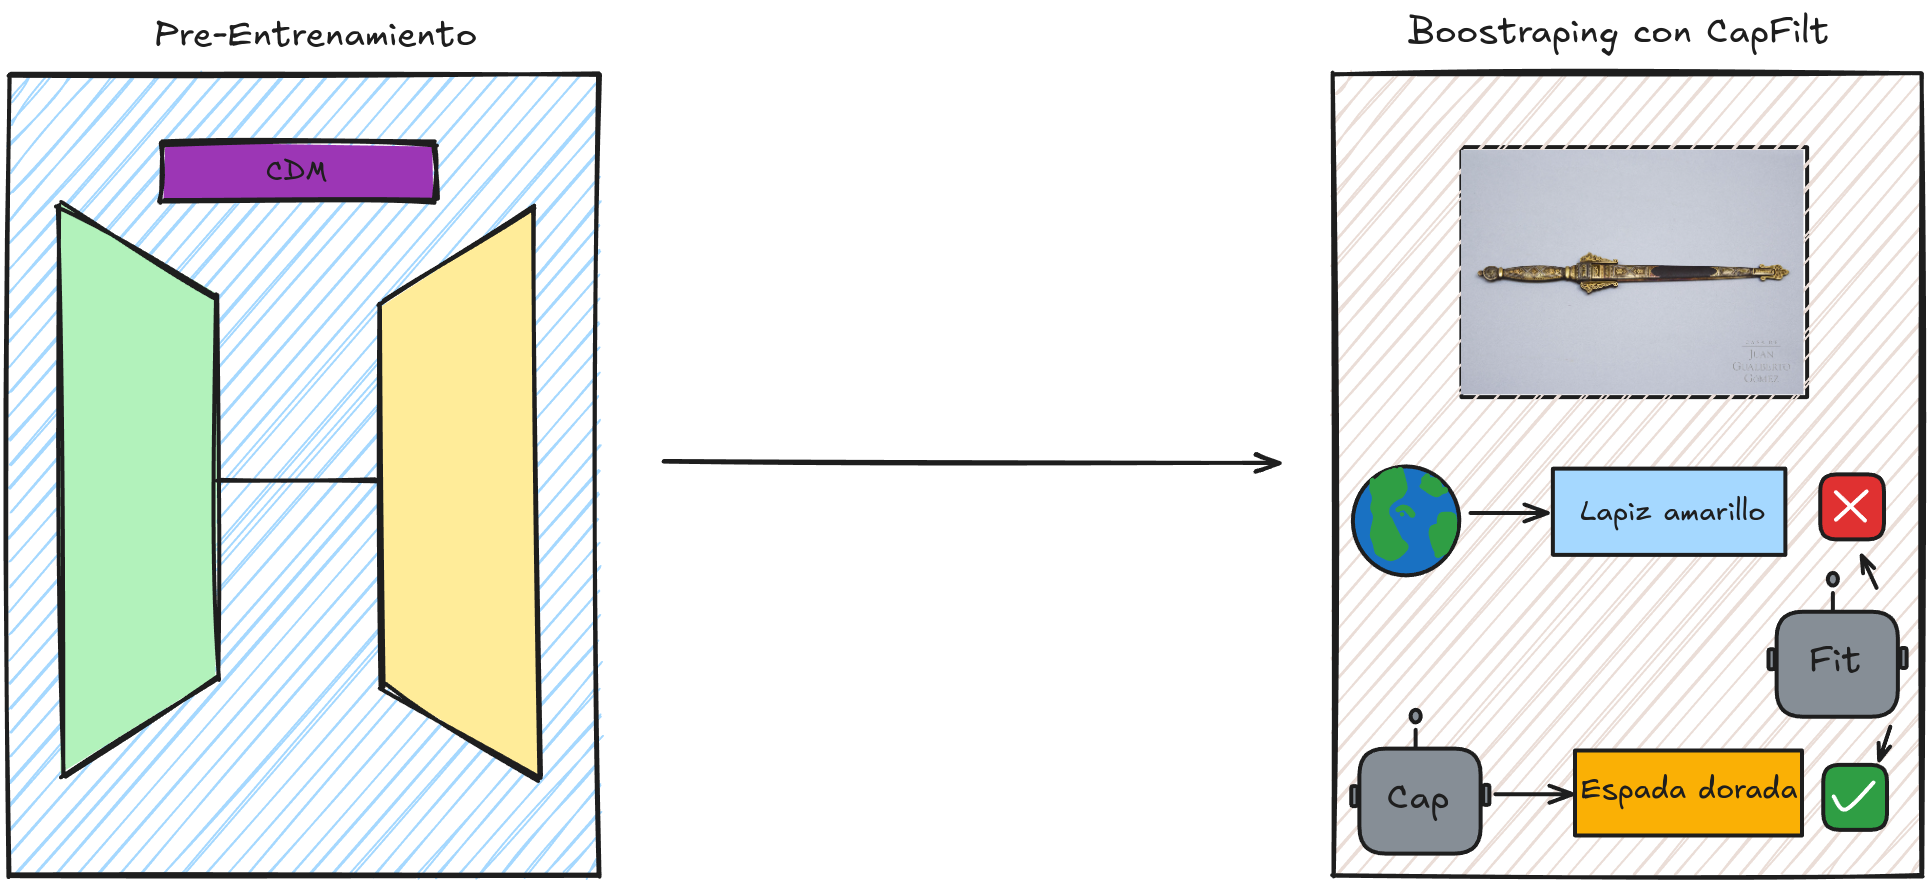
\includegraphics[width=1\textwidth]{Graphics/BLIP} 
				\caption{BLIP}
				\label{fig:BLIP}
			\end{figure}

		
	\subsection{Visual Transformers + GPT2}
	
		El modelo \textbf{Vision Transformer (ViT)} \cite{dosovitskiy2021image} está basado en la arquitectura Transformer, ampliamente utilizada en procesamiento de lenguaje natural (NLP), adaptado para tareas de visión por computadora. A diferencia de las redes neuronales convolucionales (CNNs), ViT procesa imágenes como secuencias de parches, permitiendo capturar relaciones espaciales mediante mecanismos de auto-atención.

		\subsubsection*{Arquitectura del Modelo}
			El modelo ViT se basa en los siguientes componentes fundamentales:

			\textbf{División en Parches (Patches)}
				La imagen de entrada se divide en pequeños parches de tamaño fijo $p \times p$. Cada parche actúa como una unidad similar a un token en NLP. Supongamos que la imagen original tiene tamaño $H \times W \times C$, donde $H$ y $W$ son la altura y el ancho, y $C$ es el número de canales. Al dividir la imagen en parches de tamaño $p \times p$, el número total de parches es $N = \frac{HW}{p^2}$.

			\textbf{Incrustación Lineal}
				Cada parche se aplana en un vector y se proyecta linealmente a un espacio de menor dimensión mediante una transformación lineal:
				\begin{equation}
					z_i = W E(x_i) + b,
				\end{equation}
				donde $x_i$ representa el $i$-ésimo parche, $W$ es la matriz de pesos de la proyección, y $b$ es el sesgo.

			\textbf{Incrustaciones de Posición}
				Para mantener la información espacial, se añaden incrustaciones posicionales a cada vector de parche:
				\begin{equation}
					z_i' = z_i + p_i,
				\end{equation}
				donde $p_i$ representa la posición del parche $i$ en la imagen original.

			\textbf{Token de Clasificación}
				Se introduce un token especial $z_{cls}$ al inicio de la secuencia de parches. Este token aprende una representación global de la imagen y es utilizado en la clasificación final.

			\textbf{Codificador Transformer}
				La secuencia de parches, junto con el token de clasificación, es procesada mediante un codificador Transformer. Cada bloque Transformer incluye un mecanismo de auto-atención multicabeza que permite que cada parche preste atención a otros parches en la imagen; un perceptrón multicapa, el cual transforma la representación de cada parche mediante capas densas y activaciones no lineales; y  una normalización de capa, encargada de mejorar la estabilidad del entrenamiento. Además, cuenta con conexiones residuales, las cuales facilitan el flujo de información y evitan problemas de desvanecimiento del gradiente.

		\subsubsection*{Integración con GPT2}
			El modelo ViT devuelve un conjunto de características de la imagen, las cuales se utilizan como entrada de un decodificador basado en GPT2 para obtener un texto descriptivo en lenguaje natural.

			\begin{figure}[h] 
				\centering
				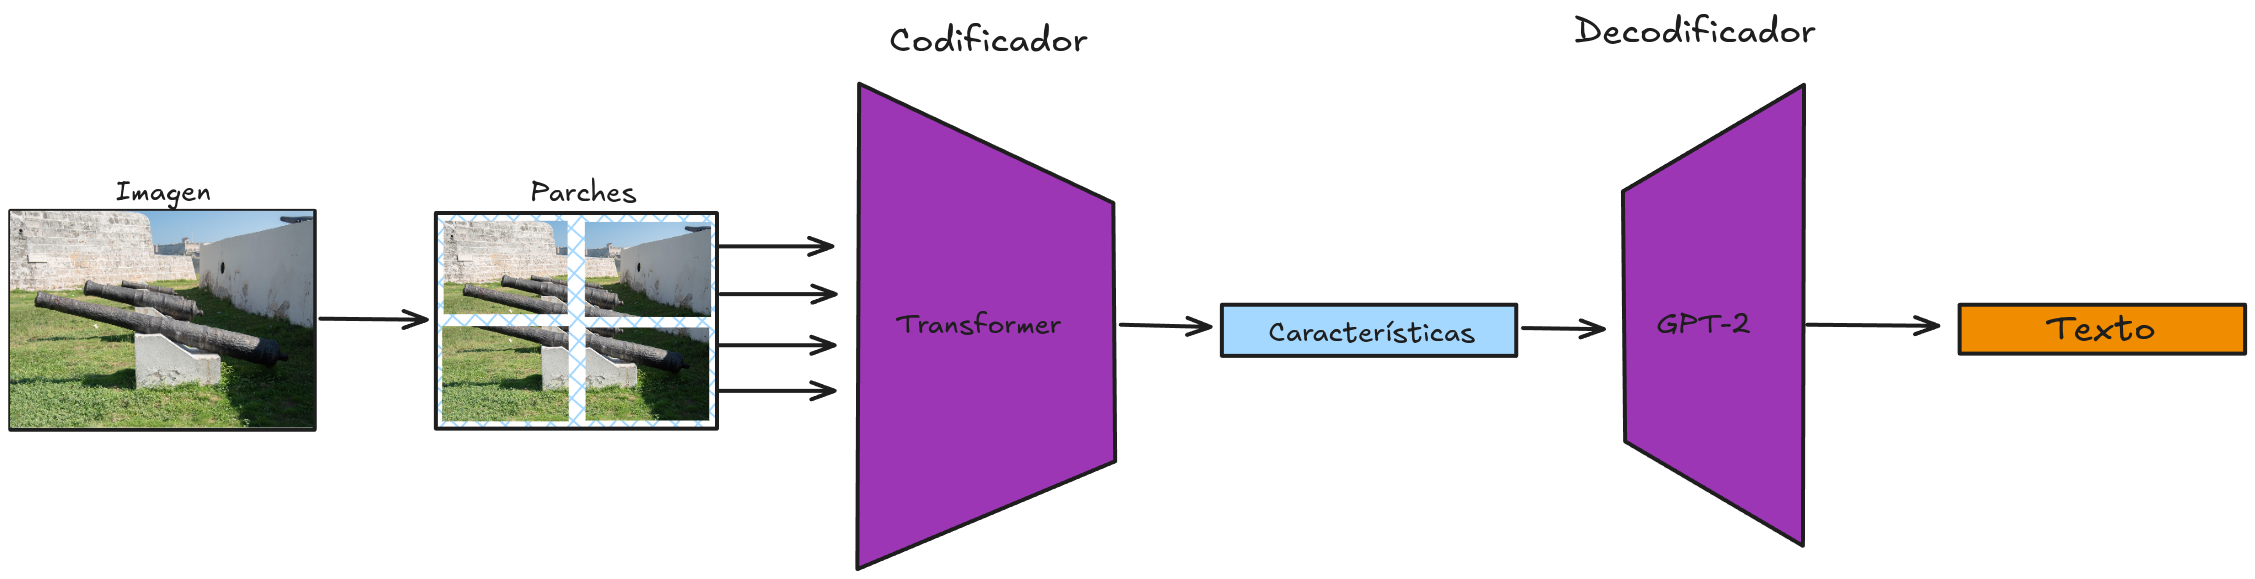
\includegraphics[width=1\textwidth]{Graphics/ViT}
				\caption{ViT}
				\label{fig:ViT}
			\end{figure}


	\subsection{CLIP}
		\textbf{CLIP} \cite{radford2021learning} es un modelo de aprendizaje profundo que permite asociar representaciones de texto e imagen en un espacio multimodal compartido. Su entrenamiento se basa en un esquema contrastivo que optimiza la similitud del coseno entre representaciones correctas y minimiza la similitud de pares incorrectos. Este enfoque permite realizar tareas como clasificación zero-shot y recuperación de imágenes a partir de descripciones textuales.

		\subsubsection*{Entrenamiento Contrastivo}
			El modelo se entrena utilizando un conjunto de datos masivo de pares imagen-texto obtenidos de la web. El procedimiento de entrenamiento sigue los siguientes pasos:
			
				 Se presenta un lote de $N$ pares $(I, T)$, donde $I_i$ representa una imagen y $T_i$ su descripción textual.
				 Se codifican las imágenes y textos utilizando un codificador de imágenes y un codificador de texto.
				 Se proyectan los embeddings generados a un espacio de representación compartido mediante una transformación lineal.
				 Se normalizan los vectores resultantes utilizando la norma $L_2$ para asegurar que todos tengan la misma escala.
				 Se calcula la similitud del coseno entre los pares $(I_i, T_j)$ generando una matriz de similitud de tamaño $N \times N$.
				 Se optimiza una función de pérdida de entropía cruzada simétrica para maximizar la similitud de los pares correctos y minimizar la similitud de los pares incorrectos.

				\begin{figure}[h] 
					\centering
					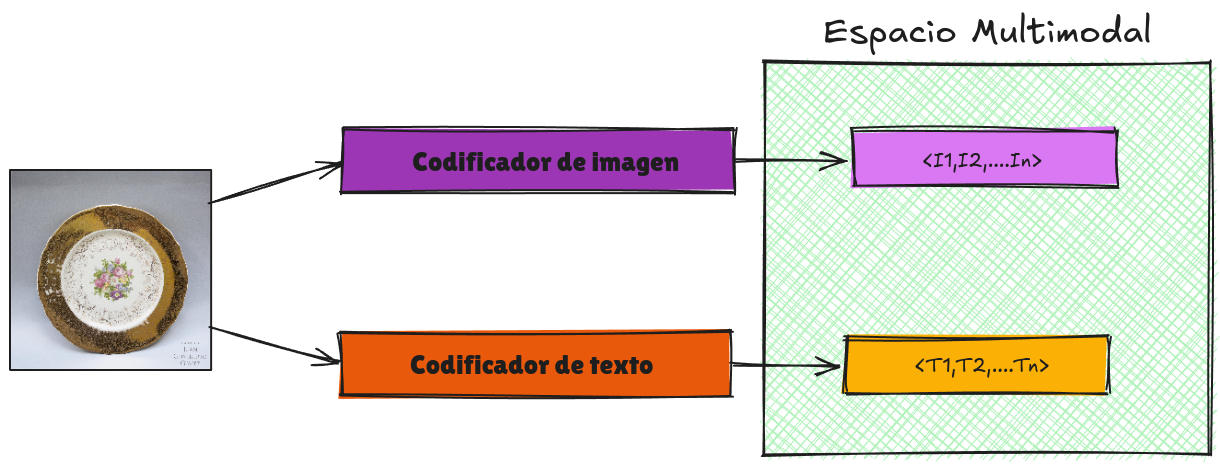
\includegraphics[width=1\textwidth]{Graphics/train_clip} 
					\caption{Entrenamiento de CLIP}
					\label{fig:CLIP}
				\end{figure}

		\subsubsection*{Codificador de Imágenes}
			CLIP emplea dos arquitecturas principales para el codificador de imágenes: ResNet modificado y Vision Transformer.
			El proceso de codificación de una imagen consiste en extraer características visuales relevantes, proyectarlas a un espacio de menor dimensión y normalizarlas para generar un vector representativo.

		\subsubsection*{Codificador de Texto}
			El codificador de texto se basa en un Transformer de 12 capas con 512 dimensiones y 8 cabezales de atención. Su procesamiento incluye tokenización del texto usando codificación de pares de bytes, adición de tokens especiales \texttt{[SOS]} y \texttt{[EOS]}, pasaje de los tokens por el Transformer, extrayendo la activación del token \texttt{[EOS]} como representación del texto, así como normalización y proyección al espacio de embedding multimodal.

		\subsubsection*{Espacio de Embedding Multimodal}
			Ambos codificadores transforman sus respectivas entradas en vectores en un espacio compartido. CLIP maximiza la similitud del coseno entre embeddings de pares imagen-texto correctos y minimiza la similitud de los incorrectos. Esto le permite generalizar a nuevas imágenes y descripciones nunca vistas durante el entrenamiento.
			
		\subsubsection*{Ejecución del modelo}
			Para seleccionar entre un conjunto de descripciones el de mayor ajuste dada una imagen, el modelo codifica la imagen y los textos con el objetivo de representar las características de los mismos en un espacio multimodal. Seguidamente, se calcula la similitud de cosenos entre los vectores de texto y el vector de la imagen, seleccionando la descripción que más se ajuste a la imagen.

			\begin{figure}[h] 
				\centering
				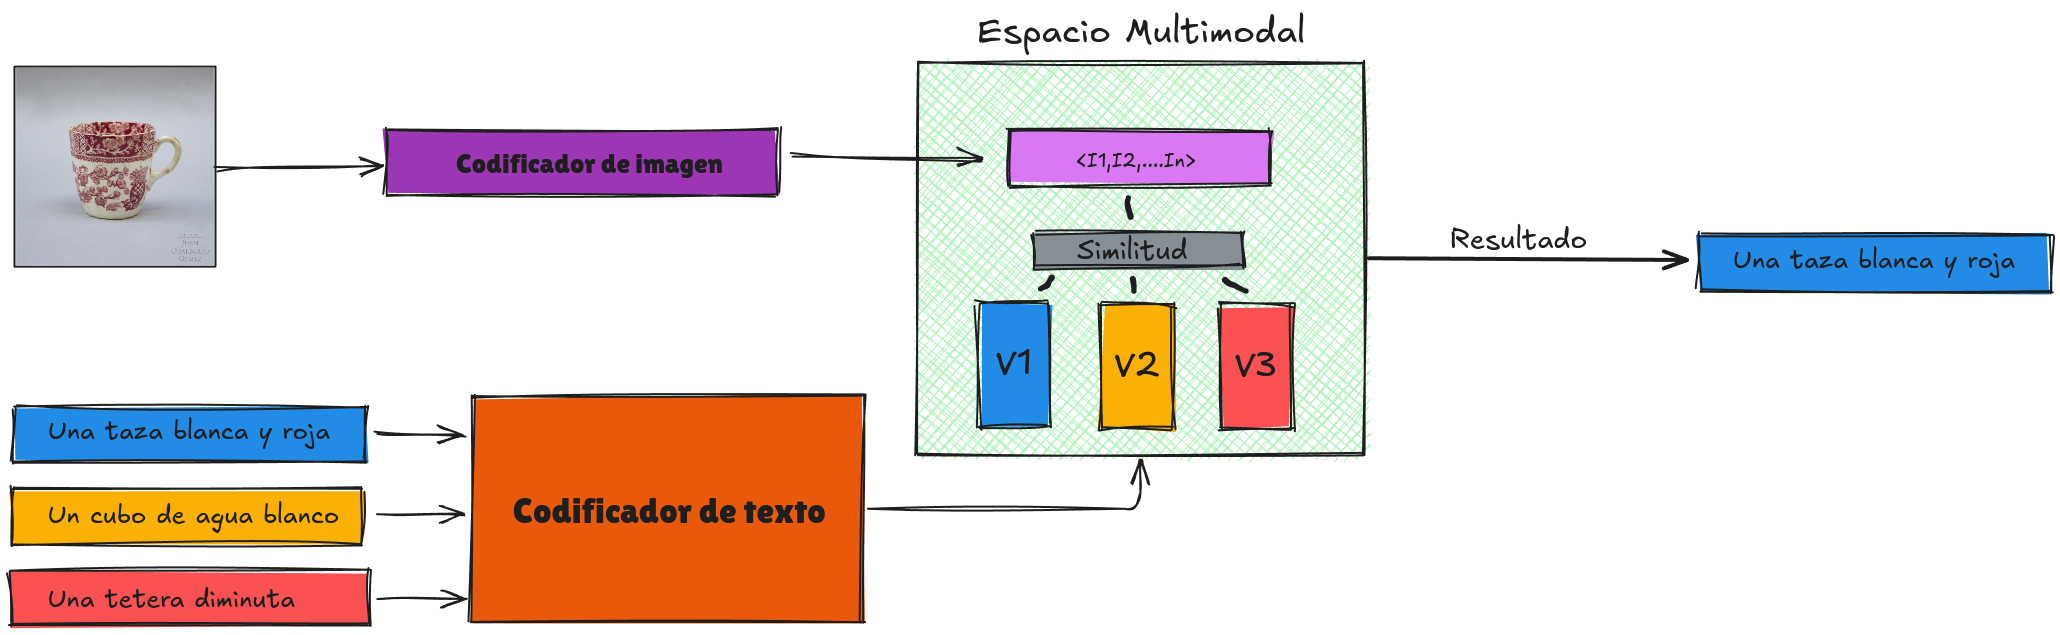
\includegraphics[width=1\textwidth]{Graphics/run_clip} 
				\caption{Ejecución del modelo CLIP}
				\label{fig:Ejecución del modelo CLIP}
			\end{figure}
